\documentclass[
    language=english,
    doctype=travel-guide,
    institution=none,
]{../../omnilatex}

\RequirePackage{config/document-settings}
\usepackage{tikz}
\usetikzlibrary{shapes, positioning, calc}

\begin{document}
\maketitle

\vspace{1cm}

\begin{center}
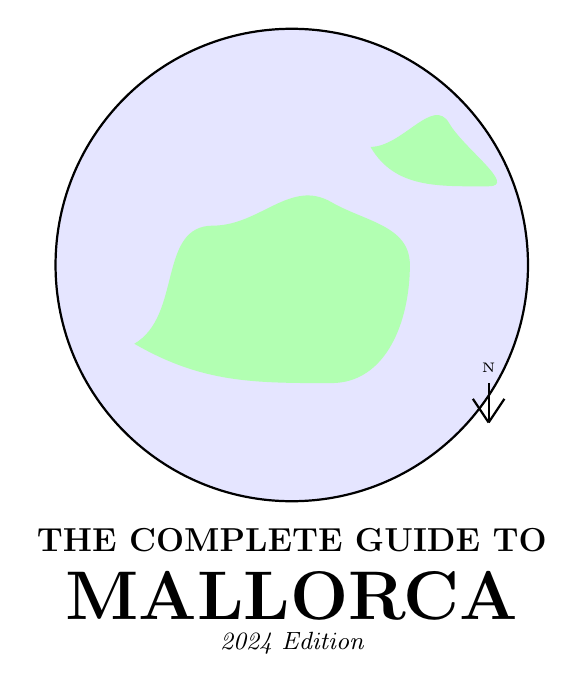
\begin{tikzpicture}
    % Map illustration
    \draw[thick, fill=blue!10] (0,0) circle (3);
    
    % Land masses
    \fill[green!30] (-2,-1) to[out=30,in=180] (-1,0.5) to[out=0,in=150] (0.5,0.8) to[out=-30,in=90] (1.5,0) to[out=-90,in=0] (0.5,-1.5) to[out=180,in=-30] cycle;
    \fill[green!30] (1,1.5) to[out=0,in=120] (2,1.8) to[out=-60,in=0] (2.5,1) to[out=180,in=-60] cycle;
    
    % Compass rose
    \draw[thick] (2.5,-2) -- (2.5,-1.5);
    \draw[thick] (2.5,-2) -- (2.7,-1.7);
    \draw[thick] (2.5,-2) -- (2.3,-1.7);
    \node[font=\tiny] at (2.5,-1.3) {N};
    
    % Title
    \node[font=\large\bfseries] at (0,-3.5) {THE COMPLETE GUIDE TO};
    \node[font=\Huge\bfseries] at (0,-4.2) {MALLORCA};
    \node[font=\small\itshape] at (0,-4.8) {2024 Edition};
\end{tikzpicture}
\end{center}

\section*{INTRODUCTION}

Mallorca is an island of contradictions. It is simultaneously one of Europe's most popular tourist destinations and one of its best-kept secrets. Beyond the all-inclusive resorts of the south coast lies a world of mountain villages, hidden coves, ancient stone villages, and a culinary tradition that rivals anything in mainland Spain.

This guide is for the traveler who wants more than a beach holiday. It is for the person who wants to climb a mountain at dawn, eat lunch in a village where no one speaks English, swim in water so clear it hurts to look at, and fall asleep to the sound of church bells and crickets.

Mallorca rewards the curious. The island reveals itself slowly, in layers, to those willing to wander beyond the obvious. This guide will help you find those layers.

\section*{GETTING THERE AND AROUND}

\subsection{By Air}
Palma de Mallorca Airport (PMI) is the island's main entry point, with direct flights from most major European cities. During peak season (June--September), flights are frequent and affordable. In shoulder season (April--May, October--November), fares increase but crowds decrease.

\subsection{By Sea}
Ferries operate from Barcelona (approximately 7 hours), Valencia (approximately 5 hours), and Denia (approximately 6 hours). The ferry is a good option if you want to bring a car, though driving in Mallorca requires patience and a willingness to navigate narrow mountain roads.

\subsection{Getting Around}

\begin{table}[h]
\centering
\begin{tabular}{p{3cm}p{5cm}p{4cm}}
\toprule
\textbf{Transport} & \textbf{Best For} & \textbf{Notes} \\
\midrule
Rental car & Exploring the island freely & Essential for mountain villages; book in advance in summer \\
Bus (TIB) & Budget travel between towns & Reliable but limited schedules; buy a BonoBus card \\
Train & Palma to S\'{o}ller & Scenic; the wooden train from 1912 is an experience itself \\
Bicycle & Flat coastal areas & E-bikes recommended for hills; Mallorca is a cycling paradise \\
Taxi & Short trips, late nights & Metered; tip not expected but appreciated \\
\bottomrule
\end{tabular}
\caption{Transportation options}
\end{table}

\section*{THE NORTH: TRAMUNTANA MOUNTAINS}

The Serra de Tramuntana is a UNESCO World Heritage Site and the backbone of the island. This mountain range runs from Andratx in the southwest to Pollen\c{c}a in the northeast, offering some of the most dramatic landscapes in the Mediterranean.

\subsection{Valldemossa}

A village of stone houses and narrow streets, perched at 400 meters above sea level. Chopin spent a winter here in 1838, and the Charterhouse monastery where he stayed is now a museum. The village is beautiful in any season, but especially in autumn, when the almond trees turn gold and the light takes on a quality that photographers call ``liquid.''

\textbf{Don't miss:} The Sunday market, the monastery, and a walk along the old cobbled path to Dei\`{a}.

\textbf{Eat at:} Ca n'Ela (traditional Mallorcan, reserve ahead), or Vila Ca n'Ela (tapas with mountain views).

\subsection{Dei\`{a}}

The most photographed village in Mallorca, and for good reason. Dei\`{a} sits in a valley between two mountain ridges, its stone houses tumbling down the hillside toward the sea. Robert Graves lived here for decades, and his house is now a museum.

\textbf{Don't miss:} The walk from Dei\`{a} to the beach at Cala Dei\`{a} (45 minutes, steep but worth it). The sunset from the cemetery viewpoint.

\textbf{Eat at:} Ca Lloren\c{c} (in the village square; excellent seafood), or Ses Escales (at the beach; simple grilled fish).

\subsection{S\'{o}ller}

A larger town in a valley of orange groves, connected to Palma by a vintage wooden train that chugs through two tunnels and over viaducts. S\'{o}ller has a beautiful main square, a decent museum, and access to the beach at Port de S\'{o}ller.

\textbf{Don't miss:} The wooden train (allow 1 hour each way), the orange museum (yes, really), and a walk through the orange groves in late autumn when the fruit is hanging heavy on the trees.

\textbf{Eat at:} Ca n'Aixa (paella and rice dishes), or Sa Fona (traditional cuisine in a 14th-century building).

\section*{THE EAST: COVES AND BEACHES}

The east coast of Mallorca is defined by its coves---small, sheltered bays with turquoise water and white sand. The best coves require a bit of effort to reach, which keeps the crowds manageable.

\subsection{Cala Mondrag\'{o}}

A protected natural park with two beaches separated by a rocky headland. The water is shallow and warm, perfect for families. There's a chiringuito (beach bar) serving grilled sardines and cold beer.

\textbf{Best time to visit:} Early morning, before the tour buses arrive. Or late afternoon, when the light turns golden and the beach empties out.

\subsection{Cala Figuera}

A working fishing village with a small beach and a harbor full of traditional llaut boats (the wooden fishing boats that are a symbol of Mallorca). The village is not on the tourist trail, which makes it a perfect place to sit on the harbor wall and watch the fishermen unload their catch.

\textbf{Eat at:} Can Costa (family-run, fresh fish, no menu---they tell you what's good today).

\subsection{Cala Varques}

A beach accessible only by boat or a 30-minute walk through pine forest. The walk is worth it: Cala Varques is one of the most beautiful beaches in the Mediterranean, with fine white sand and water so clear you can see the fish from the shore.

\textbf{How to get there:} Walk from the parking area at Cala Rom\`{a} (follow the signs), or take a boat from Portocristo.

\section*{THE SOUTH: BEYOND THE RESORTS}

The south coast is where most tourists go, but even here there are hidden corners if you know where to look.

\subsection{Cap de Ses Salines}

The southernmost point of the island, where the land tapers to a rocky point and the lighthouse stands sentinel over the meeting of the Mediterranean and the Atlantic. The drive out is flat and boring, but the landscape at the end is stark and beautiful---salt flats, scrubby vegetation, and the endless blue of the sea.

\textbf{Don't miss:} The walk to the lighthouse, the birdwatching at the salt flats (flamingos in winter), and the sunset, which is spectacular.

\subsection{Es Trenc}

Mallorca's most famous beach, and deservedly so. Two kilometers of fine white sand, backed by dunes and pine forest, with water that ranges from pale green to deep blue. It can be crowded in summer, but the beach is long enough that you can always find a quiet spot if you walk far enough.

\textbf{How to avoid crowds:} Go in May or September. Or walk to the far end, past the restaurant, where the beach becomes nudist and significantly less populated.

\section*{PALMA: THE CAPITAL}

Palma is a proper city---walkable, cultural, with excellent restaurants and a beautiful old town that deserves more than the day trip most visitors give it.

\subsection{What to See}

\begin{itemize}
    \item \textbf{La Seu} --- The cathedral, a Gothic masterpiece that took nearly 400 years to build. Gaud\'{i} contributed to the restoration in the early 1900s. The light through the rose window in the afternoon is extraordinary.
    \item \textbf{Bellver Castle} --- A 14th-century circular castle on a hill above the city, with panoramic views. The museum inside is small but worth the climb.
    \item \textbf{Mercat de l'Olivar} --- The central market, where you can buy everything from olives to octopus to saffron. Best visited on a weekday morning, when the vendors are relaxed and the tourists haven't arrived.
    \item \textbf{Old Town} --- Get lost in the streets. The area around the cathedral is beautiful but touristy; the streets east of the market are quieter and more interesting.
\end{itemize}

\subsection{Where to Eat}

\begin{table}[h]
\centering
\begin{tabular}{p{3cm}p{4cm}p{4cm}}
\toprule
\textbf{Restaurant} & \textbf{Style} & \textbf{Price Range} \\
\midrule
Ca n'Ela & Traditional Mallorcan & Moderate \\
Forn de Sant Joan & Mediterranean & Moderate \\
Mercat Vell & Fine dining & Expensive \\
Bar Bosch & Tapas, since 1932 & Budget \\
El Camino & Steakhouse & Expensive \\
\bottomrule
\end{tabular}
\caption{Palma dining recommendations}
\end{table}

\section*{FOOD AND DRINK}

Mallorcan cuisine is Mediterranean at its best: fresh, simple, and built around local ingredients.

\subsection{Must-Try Dishes}

\begin{itemize}
    \item \textbf{Pa amb oli} --- Bread rubbed with tomato and drizzled with olive oil. The foundation of every Mallorcan meal.
    \item \textbf{Frit mallorqu\'{i}} --- A stir-fry of offal, potatoes, and peppers. Not for the faint-hearted, but delicious.
    \item \textbf{Sopes mallorquines} --- A thick vegetable soup with bread. Hearty and comforting.
    \item \textbf{Sobrassada} --- A cured sausage made with paprika. Spread it on bread and eat it with a glass of wine.
    \item \textbf{Ensaïmada} --- A spiral pastry filled with cream, pumpkin, or nothing at all. Perfect with coffee.
\end{itemize}

\subsection{Wine}

Mallorca has a small but excellent wine industry. The best known denominations are Binissalem and Pla i Llevant. Look for wines from Bodega Son Puig, Son Prim, or Maci\`{a} Batle.

\section*{PRACTICAL INFORMATION}

\begin{table}[h]
\centering
\begin{tabular}{lr}
\toprule
\textbf{Currency} & Euro (EUR) \\
\textbf{Language} & Catalan (Mallorqu\'{i}) and Spanish \\
\textbf{Time zone} & CET (UTC+1) \\
\textbf{Electricity} & 230V, Type F plugs \\
\textbf{Water} & Tap water is safe but tastes of chlorine; bottled is cheap \\
\textbf{Tipping} & Not expected; round up or leave small change \\
\textbf{Emergency} & 112 (EU-wide) \\
\bottomrule
\end{tabular}
\caption{Quick reference}
\end{table}

\section*{WHEN TO GO}

\begin{table}[h]
\centering
\begin{tabular}{p{3cm}p{4cm}p{4cm}}
\toprule
\textbf{Season} & \textbf{Weather} & \textbf{Crowds} \\
\midrule
Spring (Apr--May) & Warm, 18--24°C & Low \\
Summer (Jun--Aug) & Hot, 28--35°C & Very high \\
Autumn (Sep--Oct) & Warm, 20--26°C & Moderate \\
Winter (Nov--Mar) & Cool, 12--17°C & Very low \\
\bottomrule
\end{tabular}
\caption{Seasonal overview}
\end{table}

\section*{FINAL THOUGHTS}

Mallorca is an island that rewards repetition. The first time you visit, you'll see the highlights---the cathedral, the beach, the mountains. The second time, you'll go deeper---the hidden villages, the family-run restaurants, the walks that aren't in any guidebook. The third time, you'll start to understand why people move here and never leave.

The island is not without its problems---overdevelopment, overtourism, water scarcity---but beneath the surface, there is a Mallorca that remains wild, beautiful, and deeply itself. This guide is an invitation to find that Mallorca.

\begin{quote}
\textit{``The island is a mirror. What you find there depends on what you bring.''}\\
--- Mallorcan proverb
\end{quote}

\end{document}
